\documentclass[../main]{subfiles}
\graphicspath{{\subfix{../Images/}}}

\begin{document}

\section*{Załącznik nr 1: System wbudowany}\addcontentsline{toc}{section}{Załącznik nr 1: System wbudowany}\label{sec:zalacznik-1}

Skoro nie ma jednoznacznej definicji pojęcia "system wbudowany" - należy określić definicję, która jest
wykorzystywana w tej pracę.

System wbudowany jest systemem, to znaczy ma cechy systemu: jest złożony z więcej niż jednego elementu,
jest funkcjonalnie niezależny od środowiska (tzn. może być wyodrębniony ze środowiska) i posiada
możliwość reagowania (tzn. odbierania, przetwarzania i odpowiedzi) % TODO: odbierania? możliwość?
na bodźce zewnętrzne. "wbudowany" oznacza, że system jest częścią innego systemu fizycznie i/lub
funkcjonalnie.

Natomiast przełożyć tą definicję na dziedzinę elektroniki i informatyki można w następujący sposób:
system wbudowany — jest to system komputerowy składający się z jednostki obliczeniowej i modułów
wejścia/wyjścia (tzn. może reagować na bodźce zewnętrzne), mający wszystkie narzędzia (w tym
oprogramowanie) dla spełnienia pewnej, zdefiniowanej funkcji (więc może być wyodrębniony) i będący
częścią większego systemu.
% TODO: Nie cytuję tu rzadnej książki ani normy, bazuję sie na swojej wiedzę, ale agólnie ta definicja jest podobna od książki do książki.

\section*{Załącznik nr 2: ARM TrustZone}\addcontentsline{toc}{section}{Załącznik nr 2: ARM TrustZone}\label{sec:zalacznik-2}
\begin{figure}
    \centering
    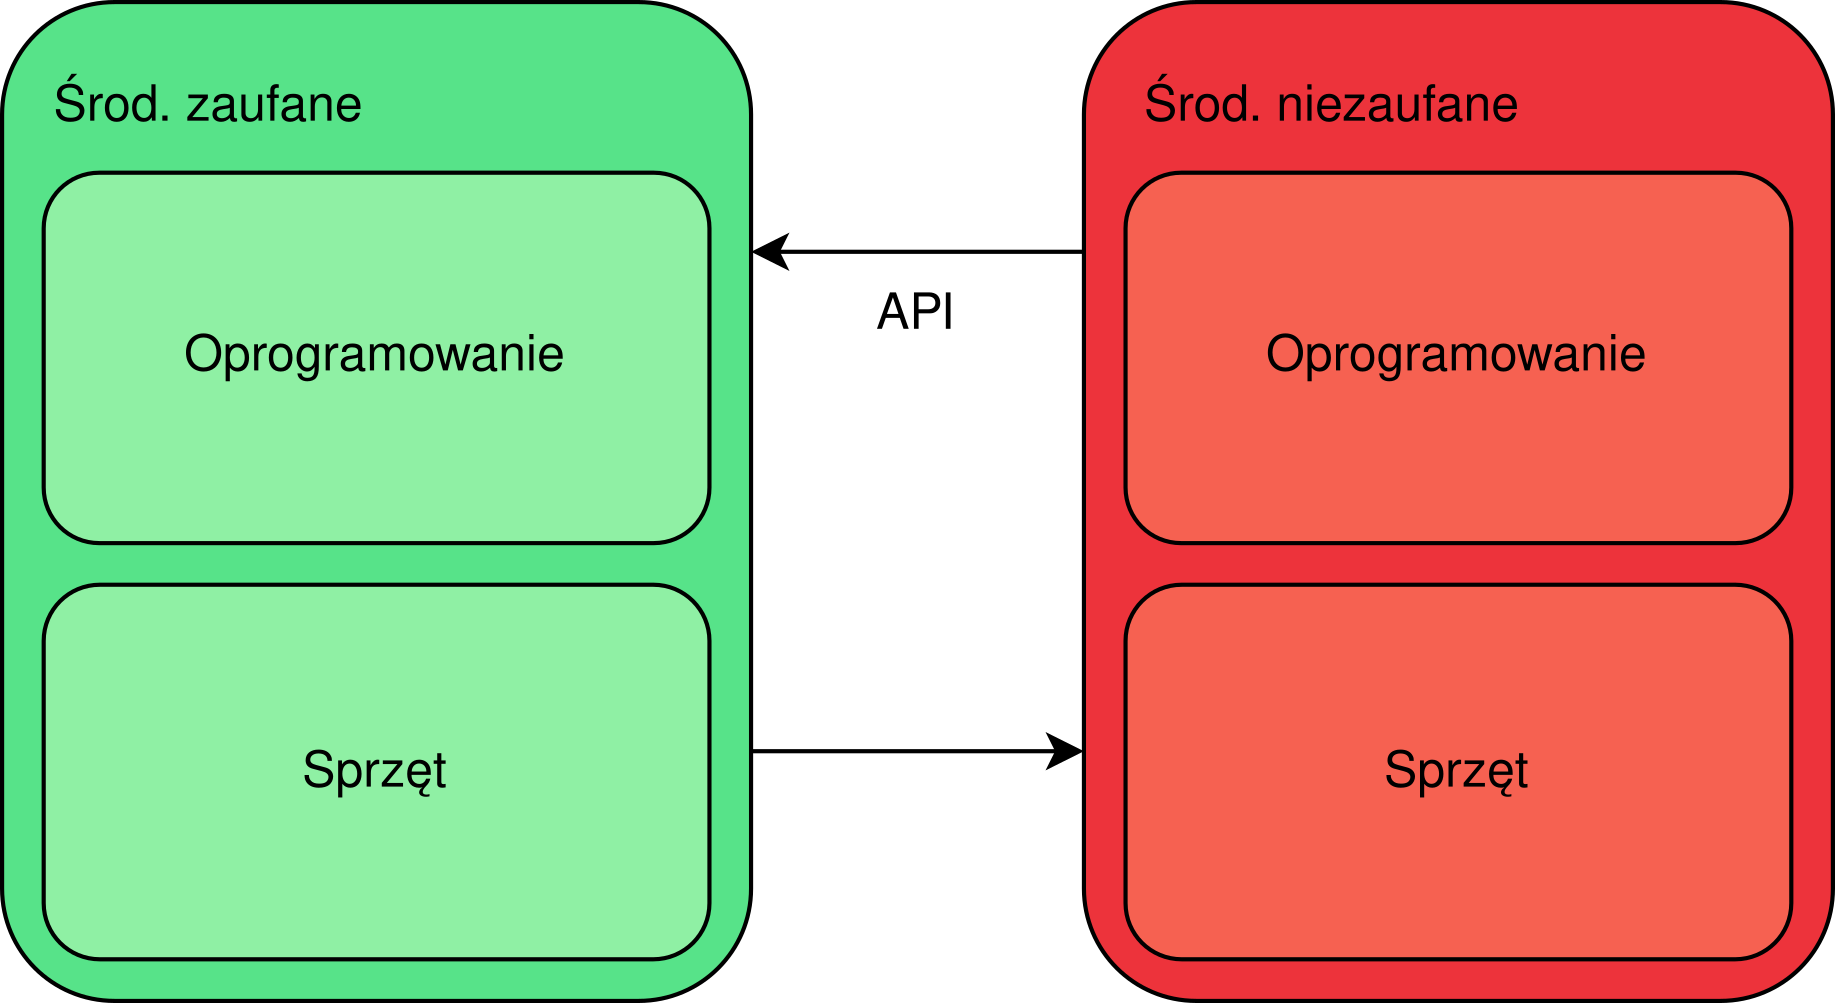
\includegraphics[width=0.95\textwidth]{Images/trustzone-m.png}
    \caption{TrustZone dla architektury \acrshort{arm} v8-M}
    \label{fig:trustzone-m}
\end{figure}
\begin{figure}
    \centering
    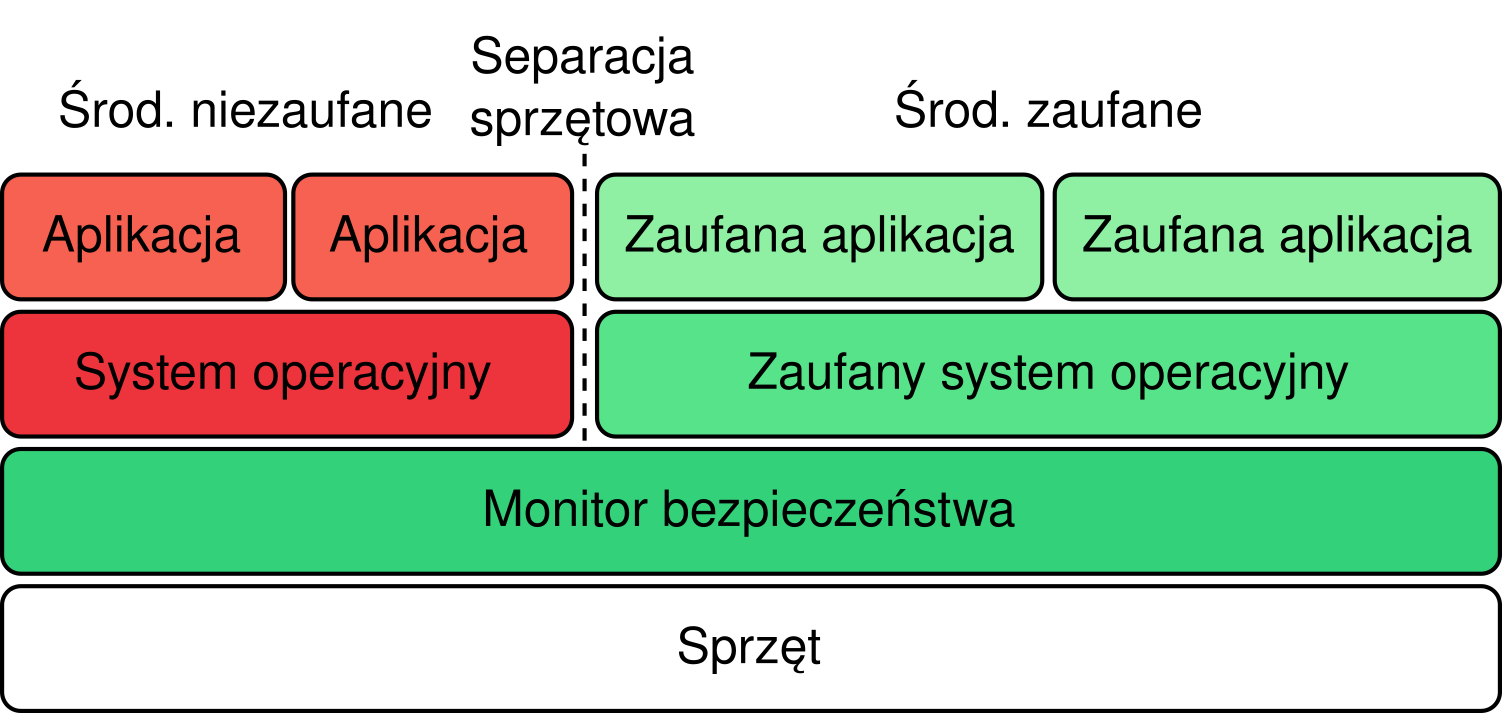
\includegraphics[width=0.95\textwidth]{Images/trustzone-a.png}
    \caption{TrustZone dla architektury \acrshort{arm} v8-A}
    \label{fig:trustzone-a}
\end{figure}

Koncept technologi TrustZone bazuję się na podziale sprzętowym środowiska (pamięci i innych zasobów) na
środowisko zaufane i niezaufane (\cref{fig:trustzone-m} i
\cref{fig:trustzone-a}), co jest robione za pomocą rozszerzeń do architektur ARMv8-A i
ARMv8-M dotyczących \acrshort{bsa} i \acrshort{isa}.

Dla architektury ARMv8-A został dodany \acrshort{el}3, w którym jest zamieszczony monitor bezpieczeństwa
(\cref{fig:trustzone-a}), realizowany przez oprogramowanie \acrshort{arm}'owe Trusted
Firmware A (referencyjna implementacja monitoru bezpieczeństwa). Faktycznie ten monitor bezpieczeństwa
jest pewnym mostem przekazującym polecenia ze środowiska niezaufanego do środowiska zaufanego oraz
przełączający procesor w bezpieczny tryb za pomocą \acrshort{smccc}.
\cite{smccc}\cite{trustzoneaarch64} % TODO: automatic images indexing

Dla architektury ARMv8-M zostały dodane rozszerzenia pozwalające na separację środowiska zaufanego od
niezaufanego (\cref{fig:trustzone-m}) za pomocą modułów \acrshort{sau} i \acrshort{idau},
oraz instrukcji dla komunikacji pomiędzy środowiskami: \acrshort{isa} SG, BXNS i BLXNS.
\cite{trustzonearmv8m}

\section*{Załącznik nr 3: Wirtualizacja}\addcontentsline{toc}{section}{Załącznik nr 3: Wirtualzacja}\label{sec:zalacznik-3}

Wirtualizacja jest technologią wprowadzającą separację środowisk z oprogramowaniem poprzez tworzenie
tzw. \acrshort{vm} zarządzanych przez \acrshort{vmm} (\cref{fig:virt}). Typy separacji używane w
wirtualizacji: separacja pamięciowa (poprzez translację pamięci), separacja sygnałowa (przekierowywanie
przerwań) i separacja stanów (przełączanie kontekstu).

Celą separacji pamięciowej jest przypisanie do każdej \acrshort{vm} przedziału adresu pamięci (kodu
programu i urządzeń peryferyjnych, ponieważ rejestry tych urządzeń są zmapowane do pamięci; ang. memory
mapped peripherals) i wychwytywanie wszystkich prób manipulacji pamięcią nieprzypisaną do tej
\acrshort{vm}. W architekturach \acrshort{arm} tym się zajmuje \acrshort{mmu}, który, zaczynając od
\acrshort{arm}v8, posiada dwa poziomy translacji: z poziomu aplikacji (\acrshort{va}), do poziomu
systemu operacyjnego (\acrshort{ipa}) i do poziomu hiperwizora (\acrshort{pa}
\cite{armv8amemtranslation}).

Celą separacji sygnałowej jest podział i przekierowywanie przerwań sprzętowych pomiędzy \acrshort{vm}.
Każda \acrshort{vm} ma przepisany podzbiór urządzeń peryferyjnych za pomocą separacji pamięci, te
urządzenia mogą generować przerwania, za przekierowywanie których jest odpowiedzialny hiperwizor i
kontroler przerwań (w przypadku \acrshort{arm}'u to jest \acrshort{gic}).

Celą separacji stanów jest sprzętowy podział wykonywanych programów i przypisanie do nich pewnych
poziomów uprawnień. Dokładniej to jest opisane w \hyperref[sec:zalacznik-4]{załączniku nr 4}.

\begin{itemize}
\end{itemize}


\end{document}
